\ylDisplay{Kärbes} % Ülesande nimi
{Aigar Vaigu} % Autor
{piirkonnavoor} % Voor
{2008} % Aasta
{G 10} % Ülesande nr.
{9} % Raskustase
{
% Teema: Geomeetriline-optika
\ifStatement
Kärbes on merevaigutükis, mille murdumisnäitaja on $n=\num{1,6}$. Tüki üks pinnaosa on sfääriline kõverusraadiusega $r = \SI{3}{mm}$. Kui vaadata kärbse pead läbi selle pinnaosa, siis näib pea asuvat kõveruskeskpunkti läbival sirgel $k = \SI{5}{mm}$ sügavusel merevaigus. Kui sügaval on kärbse pea tegelikult? 

\emph{Märkus}. Kasutada väikeste nurkade lähendust $\tan \alpha \approx \sin \alpha \approx \alpha$, kus $\alpha \gg 1$ on väike nurk mõõdetuna radiaanides.
\fi


\ifHint
Kärbse näiline asukoht vastab kärbsest alguse saanud klaasist väljunud murdunud kiirte pikenduste lõikepunktile. Selle jaoks tasub vaadelda kahte kiirt: mõlemad saavad alguse kärbsest, aga üks väljub merevaigutükist pinnaga risti ja teine väikse nurga all. Edasi tuleb kiirte geomeetriat ettevaatlikult uurida ning rakendada Snelli seadust.
\fi


\ifSolution
Olgu $O$ pinna kõverusraadiuse keskpunkt ning $K$ ja $A$ vastavalt kärbse näiline ja tegelik asukoht. Allpool toodud joonis kujutab kärbsest alguse saanud kahe kiire $AB$ ja $AC$ edasist käiku. Kärbse näiline asukoht $K$ vastab kärbsest alguse saanud murdunud kiirte pikenduste lõikepunktile (joonisel $KB$ ja $KC$).

Arvestades väikeste nurkade korral kehtivat lähendust $\tan \alpha \approx \sin \alpha \approx \alpha$, võime murdumisseaduse kirjutada kujul:
\[
\frac{\sin \beta}{\sin \alpha}=n \approx \frac{\beta}{\alpha}
\]
Kolmnurkade $\triangle OCB$, $\triangle ACB$ ja $\triangle KCB$ kaudu avaldame kaare $\widehat{BC}$
\[
\gamma r=\delta a=\varphi k=\widehat{BC}.
\]
Kolmnurkade $\triangle KAB$ ja $\triangle AOB$ kaudu avaldame nurga $\angle BOC$
\[
\alpha+\delta=\gamma \quad \text { ja } \quad \beta+\varphi=\gamma.
\]

\begin{center}
	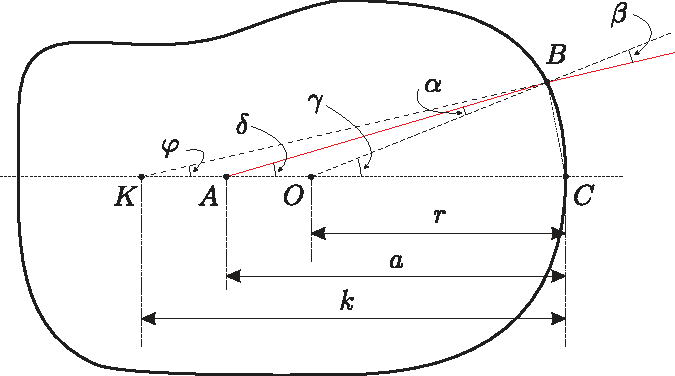
\includegraphics[width=\linewidth]{2008-v2g-10-lah}
\end{center}

Saame
\[
\begin{array}{lll}{(\gamma-\alpha) a=\gamma r} & {\Rightarrow} & {\gamma(a-r)=\alpha a} \\ {(\gamma-\beta) k=\gamma r} & {\Rightarrow} & {\gamma(k-r)=\beta k.}\end{array}
\]

Paneme tähele, et need kaks võrrandit oleks saanud otse siinusteoreemist kolmnurkade $\triangle AOB$ ja $\triangle KOB$ arvestusega, et tänu nurkade $\varphi$, $\delta$ ja $\gamma$ väiksusele $|KB| \approx k$ ja $|AB| \approx a$.

Arvestades, et $\beta /\alpha \approx n$, saame
\[
\frac{a-r}{k-r}=\frac{a}{n k} \quad \Rightarrow \quad a=\frac{n r k}{n k-k+r}=\frac{\num{1,6} \cdot \num{3} \cdot \num{5}}{\num{1,6} \cdot \num{5}-\num{5}+\num{3}}=\SI{4}{mm}.
\]
\fi
}